\chapter[System Description]{System Description}
\label{chap:system_description}

In this chapter, we will discuss the equipment used in detail, including its integration and how it was modeled and implemented in both hardware and software. 
The python automation routine that is the focus of this project was started by a previous student\cite{Monica}, and the software itself was originally created as an electrospray multipurpose library \cite{Monica}.

\section{Hardware model}
\label{sec:hardware_model}

\subsection{Instrumentation}
\label{subsec:instrumentation}

The main instruments used for this project are listed below:

\begin{enumerate}[a)]

  \item High Voltage Power Supply (HVPS)
  
     - brand: FUG
    
     - model: HCP35-20kV
    
    The HVPS provides the electrical potential to the liquid, which can be applied by connecting the HVPS directly to the liquid feeding capillary or needle to a grounded electrode (usually a plate or a ring) located downstream.\cite{Monica}
    The setup has the USB serial interface for controlling and polling measurements.
    
    The software has an interface to integrate the HVPS to our routine. This interface can be found in \emph{FUG\_function.py} file where is located the functions used to control and collect data from this instrument.
    In case of change of equipment, a new interface must be created within this file to match another manufacturer specifications.

  \item Wireless Oscilloscope
  
     - Brand: \emph{TiePie engineering}

     - model: TiePie WifiScope WS6 DIFF
    
    The signal analysis with an oscilloscope using WiFi technology allows an in-depth case study of the electric current signal.
    The current is measured via a TiePie WifiScope WS6 from TiePie engineering that is a battery powered oscilloscope capable of transmitting data via a WiFi connection allowing it to be placed in the high voltage or ground path.
    
    Wireless communication allows us to make measurements disconnected to an external power supply, which gives us more safety when using high voltage potential references and also reduce the signal noise collected from external power lines.
    The current is routed directly via the input, hence the oscilloscope measures the voltage dropped via its input resistance (which can be switched between 1 or 2 Mohms).
    TiePie WifiScope WS6 has a resolution of up to 16 bit at a minimal input range of 200 mV, sufficient to measure currents down to 1 nA.

    The interface with the software was made using the TiePie Library\cite{TiePieLib} and can be found in \emph{configuration\_tiepie.py}. Note that is also important to have the \emph{printinfo.py} file in the project folder in order to work.

  \item Humidity and Temperature sensor
  
  The stability of the system is affected by many physical effects. Evidently having the more parameters analyzed favors the system control.
  The surface tension force is dependent of the liquid-gas interface on the meniscus. Hence, the surrounding gas must be constantly the same and so its humidity.
  Also, temperature is a variable that interfere in many phenomena in the system. Specially the liquid properties such as viscosity.

  For that, a standard microcontroller development board (\emph{Arduino Uno}) with a temperature and humidity sensor (DHT11) was configured to add that data in real time in the routine.
  The Arduino code can be found in the \emph{/peripherals} folder.
  

  \item High Speed Camera 
  
  - Brand: \emph{Photron}

  - model: Photron fastcam mini


  
  \item Syringe pump
  
  - Brand: \emph{Master dual}

  - model: WPI AL-1000

  The pump integration in the automation algorithm brings us a new controllable variable, the Flow rate. Now we can control the spraying mode with the
  two main variables that affect the system. 
  It will bring more complexity for the system since now we are dealing with multivariable control.
  Controlling also the flow rate gives to this project a new dimension in the system giving us freedom to explore the flow rate properties.
  With this new input variable our control is a MISO (Multiple Inputs Single Output) system.

  About the pump interface. As I could not find a good ready-to-use library for this pump I developed a simple and intuitive interface to be our software routine.
  The communication protocol used is RS-232. In the software routine the communication used is python serial interface. The pump commands list were found in the user manual.

  % The supply at constant pressure can also favor the stability of the spray\cite{prunet}. However, the flow rate depends on the applied pressure and pressure losses between the tank and the end of the capillary, which themselves are dependent on the liquid chosen and on its temperature. This volume flow rate may also depend on the applied voltage, since the electrostatic pressure on the meniscus produces a suction effect.

  \end{enumerate}


In figure \ref{fig:setup} we illustrate a diagram with all the key components of our system. The peripherals are connected to a computer running the software routine via serial communication. 
This diagram encapsulates our process system and will be used as a sub-system in our control model. The input of our process system are power supply voltage and pump machine flow rate, referred here as the controller values. The output is the oscilloscope current sample.

\begin{figure}[H]
  \centering
  \resizebox{150mm}{!}{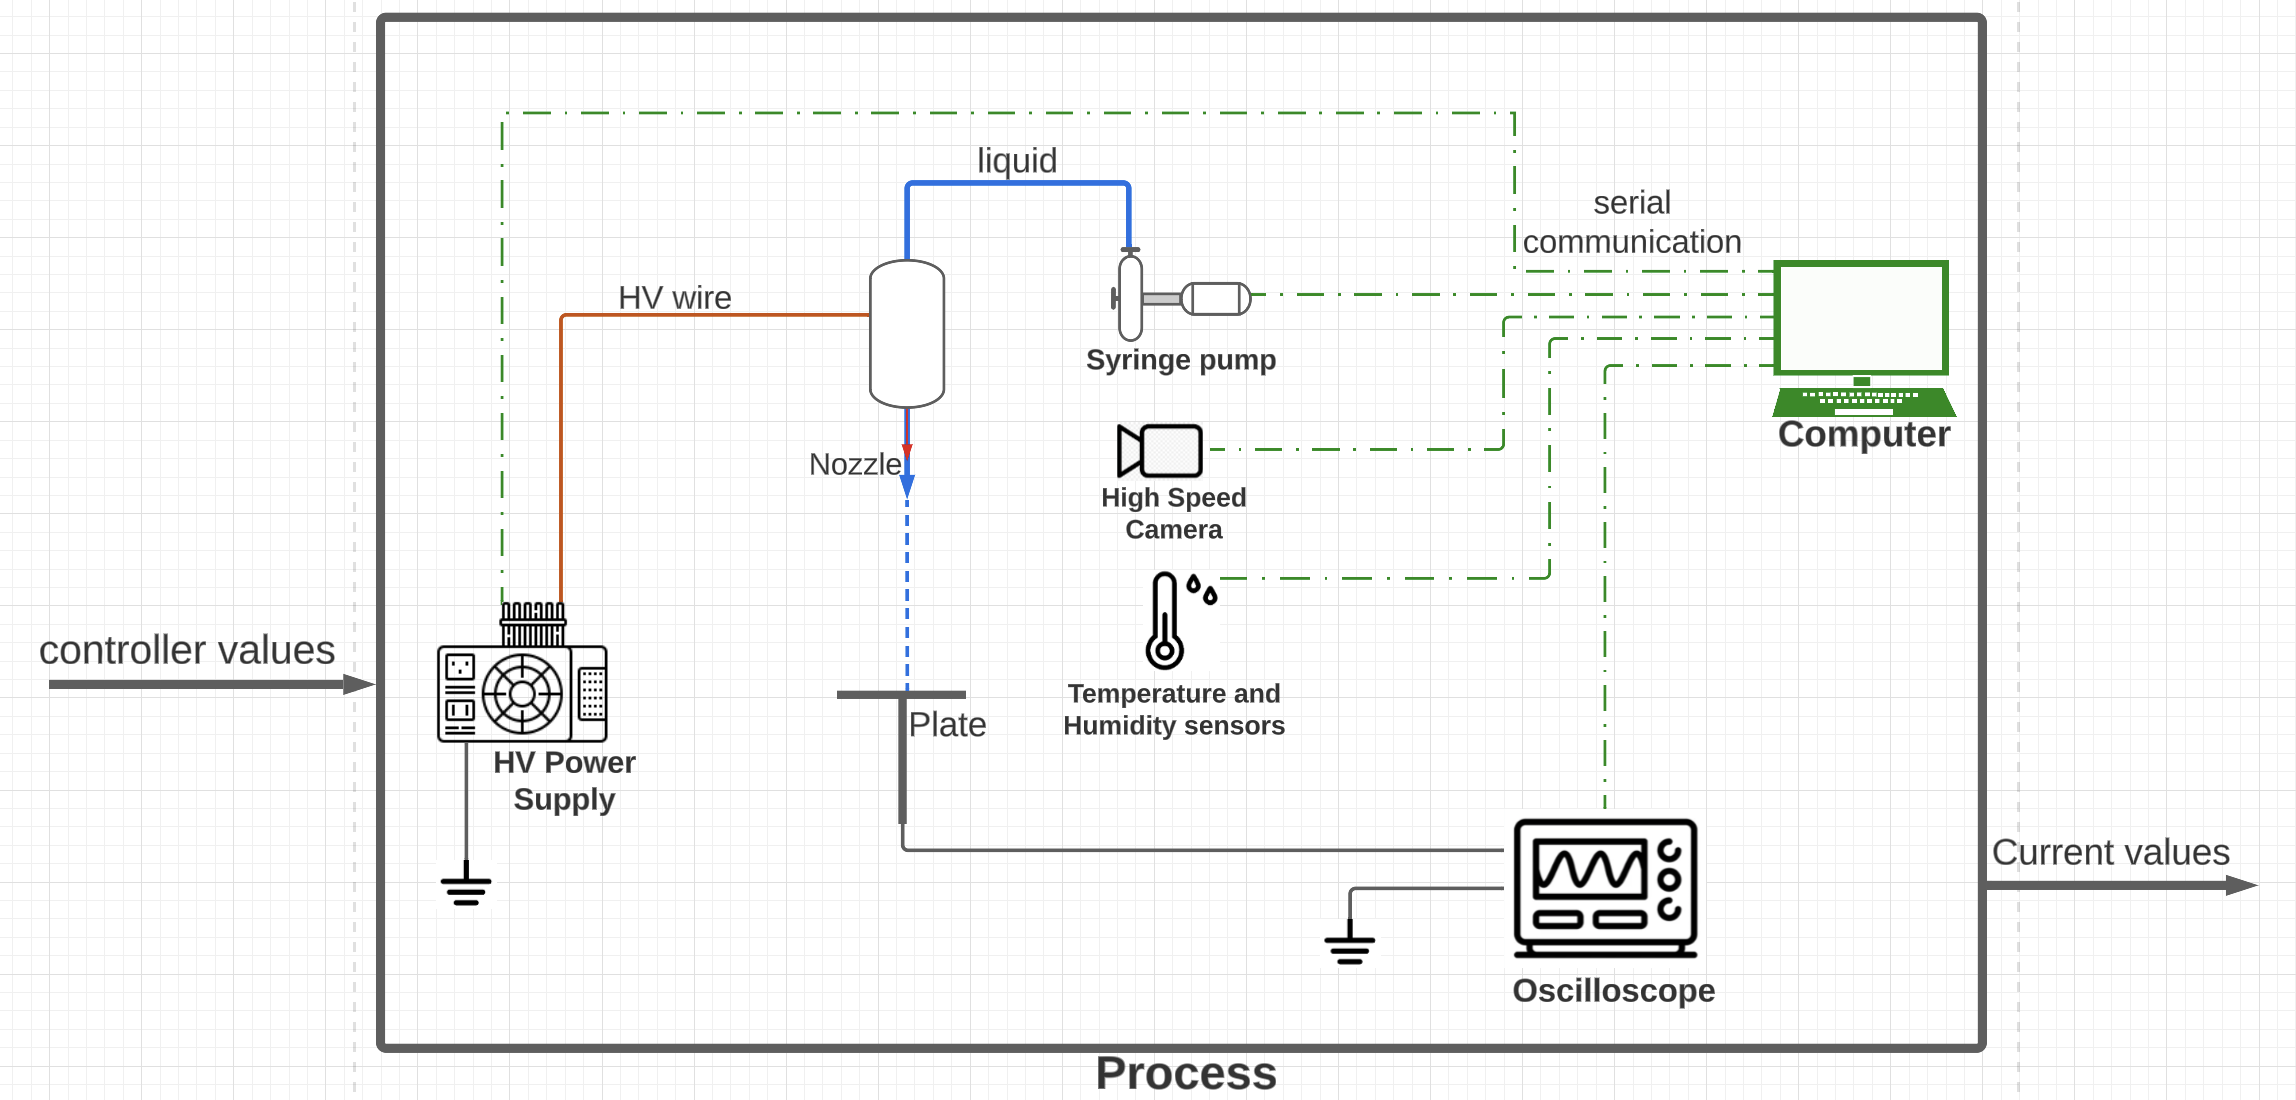
\includegraphics{Figuras/new_system_setup.png}}
  \caption{EHDA automation system setup}
  \label{fig:setup}
\end{figure}

There are also many minor variables that affects the experiment stability. More details are explained in \ref{sec:setup_validation}.


\section{Software Model}
\label{sec:control_model}

The software was reformulated on top of the control model represented in figure \ref{fig:control_model_fig}. The process of the control loop is the same as represented in \ref{fig:setup}. 
Each other subsystem in the control loop is a separate thread that will be explained bellow.

\begin{figure}[H]
  \centering
  \resizebox{150mm}{!}{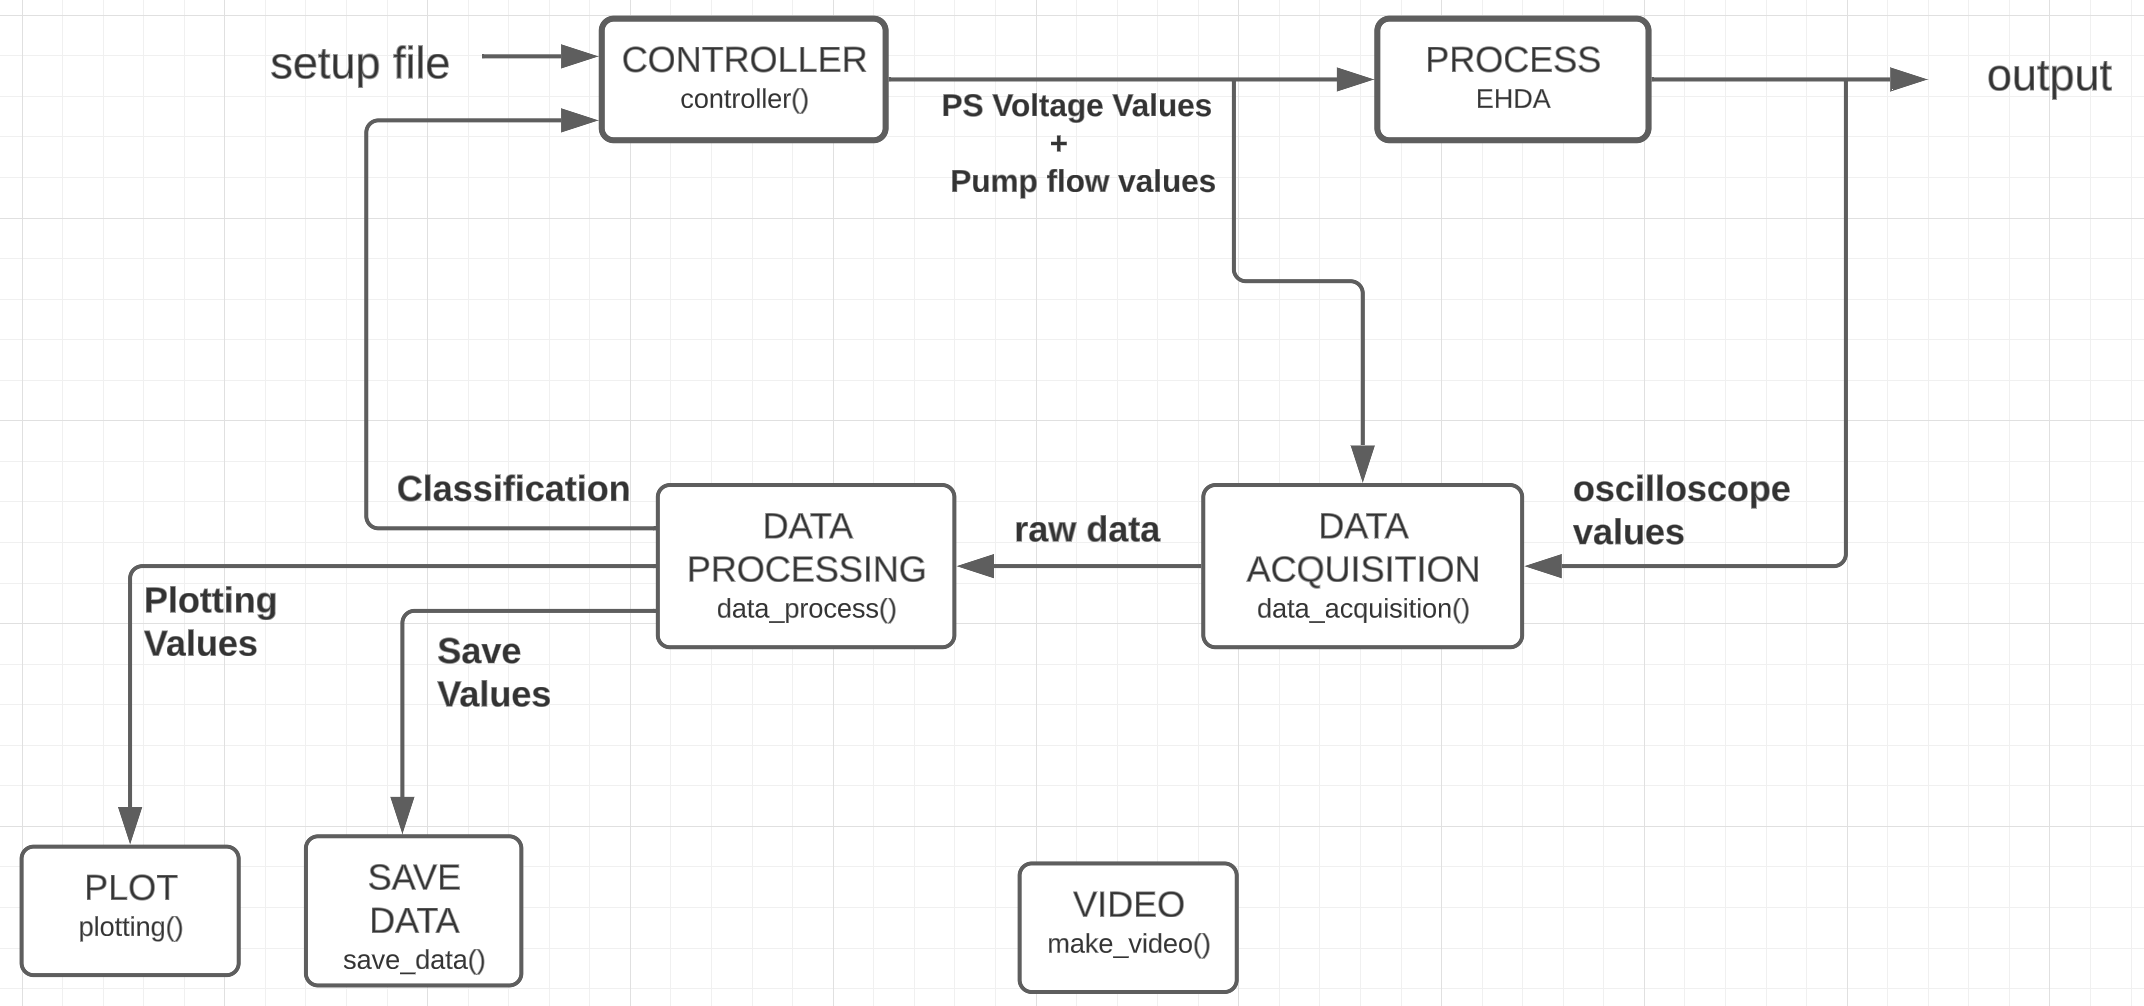
\includegraphics{Figuras/april/control_model.png}}
  \caption{EHDA automation system setup}
  \label{fig:control_model_fig}
\end{figure}

\subsection{Threading and Queues}
\label{subsec:concurrency}

    In order to implement this closed loop control model to the software and explore parallel processing, each sub-system was implemented as a separate Thread.
    For concurrency on flux of data between threads was used queues structures.
    A queue is an abstract data type that holds an ordered, linear sequence of items. You can describe it as a first in, first out (FIFO) structure.

    
    \subsection{Controller Thread}

        It is responsible for sending the power supply set voltage values and the syringe pump the flow rate set values according to the sequence selected.
        Also, responsible for sending the finish event command that end the routine and trigger the threads to close their routines.
        As input, we have the setup config file and the \emph{feedback\_queue}. As output, we have the values in the \emph{controller\_output\_queue()}.

    \subsection{Data Acquisition Thread}
    \label{subsec:data_aquisition}

        It is responsible for reading the current data from the oscilloscope, humidity and temperature data from the DHT11 sensor, voltage from the power supply, flow rate from the pump and concatenate into one sample data.
        As output, we have the values in the \emph{data\_queue()}.

    \subsection{Data Processing Thread}

        It is responsible for calculating the statistical values from the raw data and classify it in the respective spray mode for that sample.
        As output, we have the values in the \emph{save\_data\_queue()}, \emph{plotting\_queue()} and \emph{feedback\_queue()}.
    
    \subsection{Save Data Thread}
    \label{subsec:save_thread}

        After processing, the data is saved in real time in a json file using \emph{jsonstreams} library to save one sample structure at a time.
        With the new streaming model of saving a new structure of the collected data were created.
        Instead of having all data measurements values and after all data processing values we now are saving for each sample the measurements and processing values.
        The data acquired in each sample of 0.5s is shown in figure \ref{fig:data_sample}.
    
        \begin{figure}[H]
            \center
            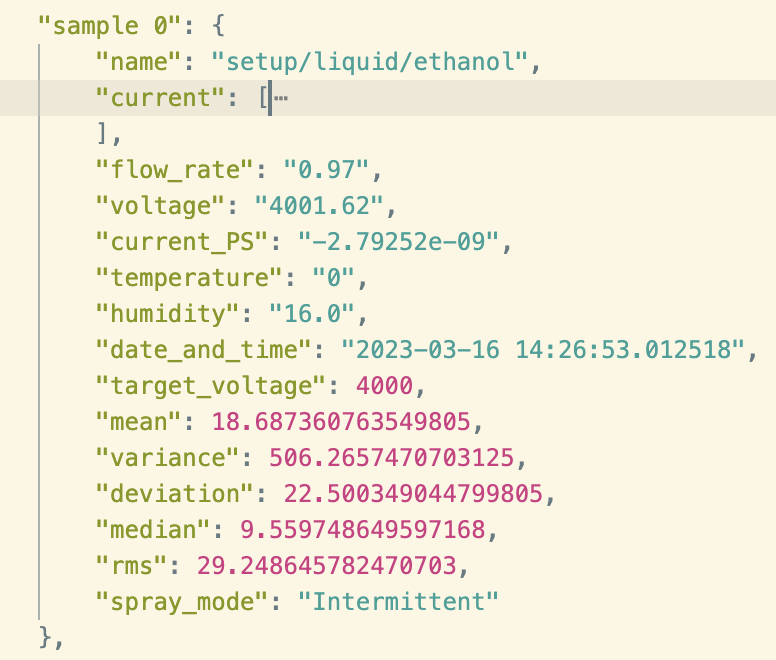
\includegraphics[width=10cm]{Figuras/19:03/new_sample.png}
            \caption{Output data json structure}
            \label{fig:data_sample}
        \end{figure}
    
        This new way of saving the measurement and processing data altogether separate by enumerated samples prevents loss of data in case of error during experiments and, specially improve in the usability of the data for further deep analysis. One experiment of around 1 hour collects around 6 GB of data. Organizing that amount of data to make it fast and easy to use was an important improvement in the software.
        To work and analyze the data we can use  pandas Data frame. A python widely used framework for data analysis.
        With the command:
        
        pandas.read\_json('PATH', orient='index').

        It will construct a Data frame with all data organized by samples.
    
        To conclude, json files are good as a system output because of its human readability. But as the database gets bigger json becomes to be a slow to read and heavy way to store the data. For that, saving the data frame in a compressed type of file called feather is much faster to work with the data.
    
    \subsection{Video Thread}

        Normally deactivated, that thread is responsible for triggering the camera in case we want to save a video of that sample.
    
    \subsection{Plot}

        The only running function that is not a thread because of the plotting library \emph{matplotlib} incompatibilities of running outside the main function. 
        It is responsible for plotting in real time the current sample acquired, and its respective fast Fourier transform to evaluate the sample frequency spectrum.
        It takes as input the \emph{plot\_data\_queue} from the \emph{processing\_thread()} and displays three graphs updated in real time on the screen during the experiment.

  \section{Chapter conclusion}

    In this chapter we described the system description detailing the hardware instruments, how it was modelled and its implementation in the software. Figure \ref{fig:metodology_example1} shows a print screen of the user interface during an experiment.

    \begin{figure}[H]
      \centering
      \resizebox{150mm}{!}{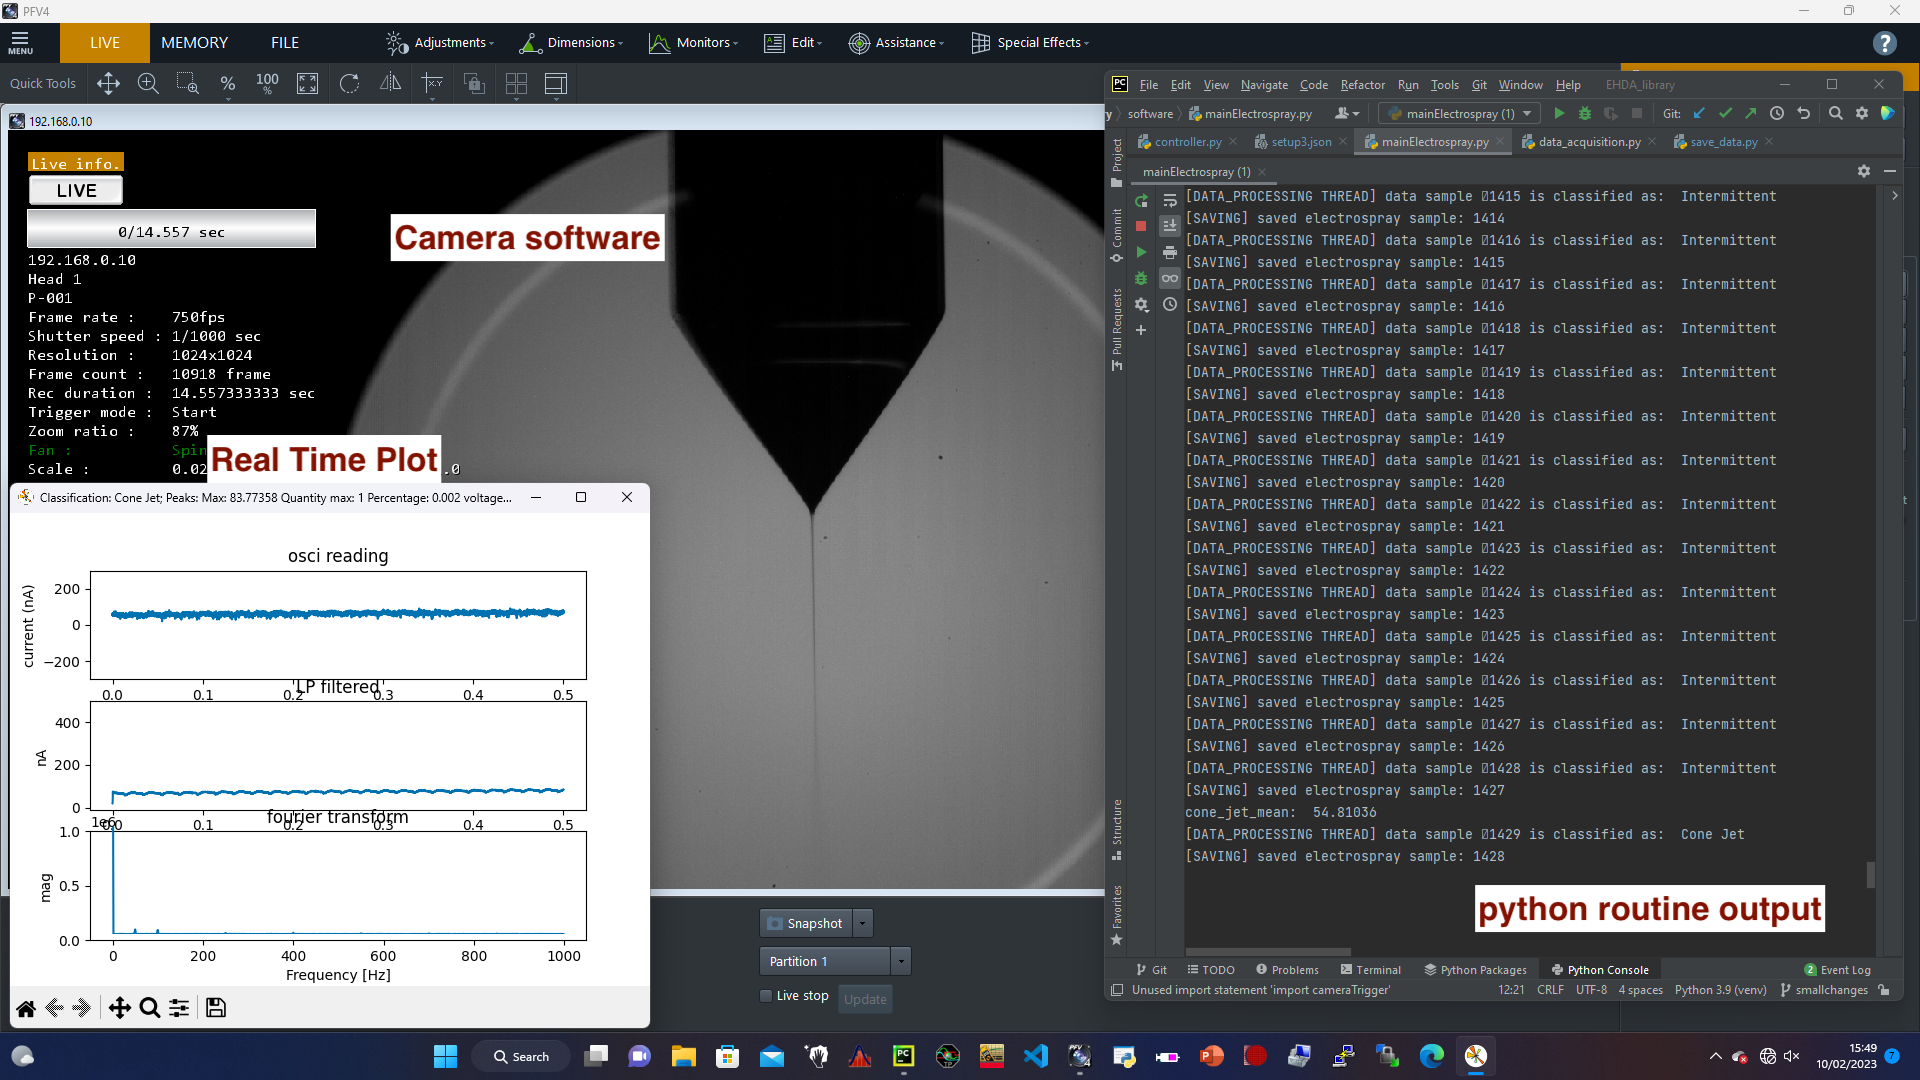
\includegraphics{Figuras/report4/experiment_print1.png}}
      \caption{EHDA automation system setup}
      \label{fig:metodology_example1}
  \end{figure}
\clearpage
